\documentclass[11pt]{report}

\title{\textbf{pyturn}\\
An Open-Source Turn-Based Battle Framework}
\author{Max Vizard | 09006863\\
		James Heslin | 09006132\\}
\date{November 23, 2012}
\usepackage[hmargin=2cm,vmargin=2cm]{geometry}
\usepackage{graphicx}
\begin{document}

\maketitle

\tableofcontents{}

\pagebreak

\section{Narrative}
You and a small team of friends have decided to construct an open-source framework/engine for turn based, party-based battle games. A sample implementation should be included to help other developers understand the framework. 

\section{Requirements}
	\subsection{Functional}
	\begin{itemize}
			\item{A system for two or more ‘parties’ of at least one character to engage in some form of turn based competition.}
			\item{Each party member takes a turn in the competition, during which they can perform set actions.}
			\item{Party members have their own individual attributes that influence their performance and possibly the turn order.}
			\item{An interface for at least one player to interact with the system, controlling one or more party members, allowing for action selection, result output and display of game state.}
			\item{A method of storing game state and predetermined gameplay variables.}
			%\item{A method of persisting game state if program is ended and allowing the player to continue from that state when the program is run again.}
	\end{itemize}
	\subsection{Non-Functional}
	\begin{itemize}
		\item{Portability}
		\item{Extensibility}
		\item{Interoperability}
		\item{Quality}
		\item{Comprehensibility}
		\item{Short development cycle}
	\end{itemize}

\section{Architectural Use Cases}
	\subsection{Asynchronous rock, paper, scissors game}
	Developer wants to create a game for two people to play the rock, paper, scissors game together on the same computer, taking turns to enter their choice and then evaluating a winner as though the choices had taken place at the same time. 
	\subsection{Monster battle game (in the style of Pok\'{e}mon\textregistered)}
	Developer wants to create a game where the player controls a group of monsters in battles with other groups of monsters. Each monster has a number of moves they can perform, but each move can only be performed a certain number of times during a single battle. Each turn, the player can choose to switch out their monster or make a move. The game is won when one player’s monsters are all incapacitated.
	\subsection{Digital implementation of trading card type games}
	Developer wants a game where players can take turns placing cards on a virtual table, similar to games like Magic: the Gathering. Cards can have various effects on either player, such as increasing or decreasing their ‘life’ score, allowing them to draw extra cards from a deck, etc.
	
\section{Design Patterns}
	\subsection{Bridge Design Pattern}
	Our project is quite a simple game framework, which makes it ideal for multiple platforms. Not wanting to clutter our logic classes with switch cases depending on platform, we researched patterns that would allow us to separate display from logic easily. The Bridge Design Pattern is a method of separating platform- or implementation-specific functionality from independent functionality. It is a good example of the software design principle, \emph{encapsulate what varies}. In the ideal case, it decouples the abstraction from the implementation altogether. One side of the 'bridge' is our independent implementation, which has a reference to an abstraction (in the form of an interface or abstract class). This is the other side of the bridge. In our independent implementation, wherever we would normally need to differ our implementation based on the variables in the system, we can instead call upon the abstraction to perform the system-specific functions. We have to trust the abstraction and its subclasses to do this. An example of where to use the Bridge pattern is in programming a game that should be playable using a terminal emulator or through a graphical window. The independent implementation might be a GameLogic abstract class, and the display abstraction a GameDisplay abstract class. The bridge separates any display code from the methods (such as \texttt{display("some text")}), which are called by GameLogic. Not only this, but the same \texttt{GameDisplay.display()} calls will display text in a terminal emulator, a GTK+ window, or whatever graphical user interface subclass is required. An alternative to the Bridge pattern is the Adaptor, which is similar, but distinct. While the Bridge has its abstraction and implementation tightly coupled, the Adaptor places another class or interface between the two, acting as an intermediary. We decided not to use the Adaptor, as more than one layer between the implementation and the abstraction is not necessary in our application. The Bridge supports our quality attributes of comprehensibility, portability, and extensibility. Keeping logic code free of out-of-band functionality like displaying text onscreen allows our code to be much more understandable. The Bridge is also inherently supportive of portability and extensibility, because it makes it easy for client developers to change or add implementations on the abstraction side.
	
	\subsection{State Design Pattern}
	Most games of any kind have multiple states, which change how they behave. The State Design Pattern aims to encapsulate those states and abstract away the different behaviours. In our game, we use the State pattern to manage the behaviour of two different scenarios: the user in the menu, before starting the game, and the user playing the game. Both states implement the same interface, allowing the main game class not to care which state is which for the purposes of getting input and displaying output. We could have used the similar Strategy pattern here, but Strategy is more useful for doing one thing than it is for modelling a scenario. The State pattern fits well in our application because it supports our quality attributes of extensibility and comprehensibility. Client developers can easily add new states to the game if they want to model additional scenarios. In addition to this, the State pattern is quite easy to understand, so it lowers the barrier to newer developers wishing to use our framework.
	
	\subsection{Delegates}
	Delegation is a method of programming to interfaces, rather than implementation. At its most basic, compositional delegation involves class A calling a method in class B, which delegates to a method in class C. Class A never knows that C exists, which keeps C's logic well-encapsulated. We use delegation a lot in our game, as it supports our non-functional requirement of code quality. Delegation allows for an application to be decomposed into modules and layers quite easily, and then for these modules and layers to call each other in a chain in order to perform a function. For example, in our game state class, we call a method that gets all the available options for the user at this particular moment. Unbeknownst to the game state class, the game engine retrieves the options from the game variables class. This also fits well with our multi-tiered architectural pattern. 

	\subsection{Decorator Pattern}
	The decorator design pattern allows developers to attach additional functionality to an object at runtime, providing a less rigid alternative to inheritance. By extending functionality while adhering to interfaces, this pattern supports the quality attribute of extensibility without compromising readability and comprehensibility. A suitable use case for this pattern exists in our system. Players can perform certain actions, which are represented by concrete subclasses of the Action class. By providing a decorator interface for this class, the framework will allow client developers to quickly and easily extend the functionality of any given action, with a variety of simple decorator classes. This will prevent subclass explosion, and may also decompose a lot of complex features into smaller, more comprehensible classes. The decorator relies on delegation to defer logical operations to another class, simplifying the operational logic of each decorator. 

	\subsection{Observer Pattern}
	The Observer Pattern is used in situations where changing one object requires changes to one or more other objects. Instead of having tight coupling between these classes, this pattern provides a flexible interface to model such a relationship. The subject is the name used to describe the class that changes state upon which one or more observers depend. The subject should be able to inform observers of changes to its state without knowledge about those classes. The observers need to define an interface for accepting updates from any subjects that it subscribes to. The term publish-subscribe is often used to describe this style of interaction. The abstract coupling of the subject and its observers allow the pattern to cross different layers of abstraction within an architectural pattern, without breaking the layered system. This is particularly relevant to our framework, where logic level classes may wish to subscribe to changes in data layer subjects. Some issues can arise with the implementation of this pattern, and so it is important to carefully consider how the pattern can be applied to the situation at hand. Due to the nature of the abstract coupling of observers, updates to the subject may incur heavy overheads due to the subsequent notification to all observers. Therefore, updates to the subject should be carefully managed. A decision should be made as to whether the subject calls notify in every mutator/state setting operation, or whether to depend on clients to call notify at an appropriate time. The flexibility of the notification process, often a useful feature of the pattern, may lead to unintended or unnecessary updates. Another issue lies in the update protocol used by the subject to notify subscribers of changes. The subject often simply passes a reference to itself to the update function of its subscribers, leaving them to infer what has changed about it. If the subject is complex, this may be labour intensive and time consuming. Therefore, it is common practise to define a Change-Manager class to carefully manage these interactions. In our project, we use the Observer pattern to publish changes to variables to the database.

	\subsection{Factory Method Pattern}
	The factory method pattern belongs the grouping of design patterns called creational patterns. These patterns are concerned with the instantiation of objects within a framework and how to maintain quality attributes such as extensibility. These patterns support the Open Closed Principle; closed for modification, open for extension. The main point of the factory method is to defer object instantiation to a method, which is left abstract so that client developers can specify which subclass of the object to instantiate when they implement the abstract class. A classic example would be a class that needs to instantiate some Product but the application designers don't know in advance what type of ConcreteProduct that may be needed. An alternative pattern is the Builder pattern which abstracts out the construction of a complex object and provides the same benefits of deferring object instantiation, albeit with more overhead. We felt that the Builder pattern was too complex for our needs and required more class definitions than was strictly necessary. 
	
\section{Deployment Options}
\begin{figure}[htp]
\centering
\includegraphics[scale=0.5]{PyturnDeploymentDiagram1.png}
\caption{Deployment Diagram}
\label{Deployment Diagram}
\end{figure}
The deployment options for this framework are extremely varied. The UML documentation should make it straightforward to realise the abstract design in most object oriented languages, despite the fact that the system was designed with Python in mind as a language platform. One of the non-functional requirements for the project was to have a short development cycle, which was the main reason for choosing Python. The language also inherently supports several other quality attributes such as readability, portability and maintainability. Python is gaining popularity and is supported on many platforms and application environments. Any platform capable of running the Python interpreter should be able to run our application, from the ARM-based Raspberry Pi to x64 Unix servers. The abstract framework and sample implementation are fully functional in Python and are both heavily documented in accordance with recommendations in Python Enhancement Proposal 8. 

The Multi tier architecture pattern that we used for the framework was chosen with the quality attributes of interoperability in mind. Organising the system into three distinct layers and carefully managing the classes that link any two layers makes it quite straightforward to deploy each layer on separate machines. By having only one class that bridges each layer gap, the work involved in integrating a transport protocol should be minimised. Several simple existing Python modules handle this type of transport in a simple and intuitive manner, which could easily integrated into an appropriate concrete sub-class. Examples include MySQLdb, Mongodb, httplib, xmlrpclib, pycurl etc. The list goes on and client developers can choose an option they would be comfortable or familiar with, depending on their needs. The bridge pattern used for the presentation layer should also make implementing a platform specific interface pretty trivial, requiring only one new detailed sub-class of GameInterface and a corresponding (simple) sub-class of GamePresentation. 

The current sample implementation of the system, ‘ElectionGame’, is designed as a standalone Python program. In this form, the program is only intended to be deployed in one place i.e the user’s PC/laptop. Any system capable of running python with standard output/input can run the program as is. This type of deployment is illustrated in Fig 1.1. In order to facilitate persistent state, some form of database backend should be added (by fully subclassing DBManager), such as SQLite. This instance would easily run currently on the same system as the program itself, even on the Raspberry Pi. This version could easily be packaged with any Linux based package manager such as RPM for distribution or simply run from source.

Should any developer wish to use the framework for much larger scale deployment, there are many Python application environments that they could choose from. In this current age of the ‘cloud’, web apps are usually the deployment platform of choice. Apart from open source solutions such as Zope, OpenStack and WSGI, there are some interesting proprietary options such as Google’s App Engine. An example of this deployment option is shown in Fig 1.2. The GAE provides a scaleable python environment based on Google’s own application platform, with numerous API’s to access their services, including their cloud storage solution GQL. The interesting thing about GAE is the payment model which is based on resource usage making for a potentially cost effective hosting solution but one that has the potential to scale to millions of users. 

A Python HTML templating system would make for a quick easy web interface implementation. The open source Python web framework provides such functionality as an individual module. The whole Django stack also makes for a quick, simple solution to a scaleable web app deployment of the framework. It provides a convenient Object Relational Mapper to create a database representation of a Python class, with pluggable database modules for several popular data stores. Django is an Model View Controller based framework, a very similar architecture to ours. Each layer of the Django stack functions as independant pluggable python modules. An example deployment based on a Django app is shown in Fig 1.3. The presentation layer is shown as a Linux based application for the Unity UI, which has a Python API. This could be switched for the standard Django web interface based on the template system.
	
\section{Use Cases}
\subsection{Use Case Diagram}
\begin{figure}[htp]
\centering
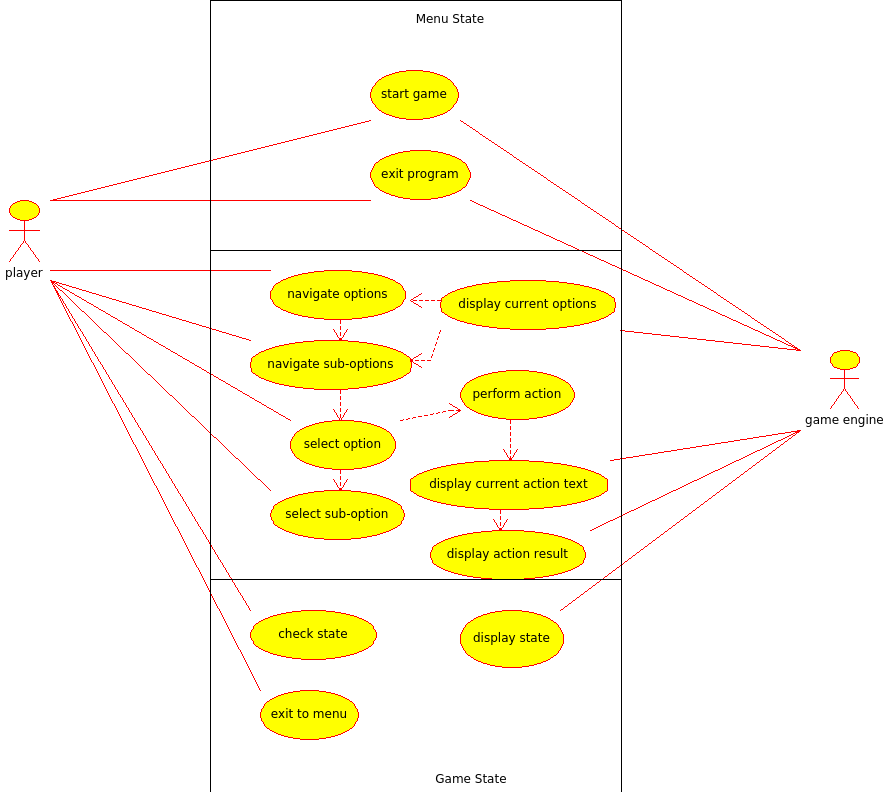
\includegraphics[scale=0.6]{PyturnUseCases.png}
\caption{Use Cases}
\label{Use Cases}
\end{figure}
\subsection{Use Case Descriptions}
Navigate Options
Description: The user needs to be able to select an action/option from a list of context specific possibilities.
Depends on: Display Options
Includes: Navigate Sub-options, Select Option

Navigate Sub-options
Description: The user also needs to be able to select an action/option from a list of context specific sub options.
Depends on: Navigate Options, Display Options
Includes:  Select Option

Select Option
User selects a possible option or action and the system should respond accordingly, either performing a game action or displaying a sub-menu.
Depends on: Navigate Options, Navigate Sub-options, Display Options
Includes: Perform Action, Display Sub-options

Perform Action
The system should perform the specific action that the user selected from the options and then output the results of that action.
Depends on: Select Option
Includes: Display Current Action Text, Display Action Result

	
\section{Architectural Analysis}
	\subsection{Multi-Tiered Architecture}
	The pattern we chose to use for our application is the Multi-Tiered Architectural Pattern. This pattern's intent is to split the application into tiers and keep the application as reusable as possible. In the application we actually use a subtype of the Multi-Tiered Architecture, Three-Tiered Architecture. Specifically, this architectural pattern splits the application into a presentation or display tier, a logic or business tier, and a database tier. We chose this pattern because in an open-source application, keeping the design modular is important. If parts of your system are to be reused by others, it is ideal to have those parts as loosely coupled as possible from logically different modules. For example, our Presentation tier is accessed only by making a call from one class in our Logic tier, to another class in the Presentation tier. The Logic tier has no other knowledge of the Presentation tier. Going in the other direction, the Data tier is only accessible through the GameplayVariables class. 
	Developing in logically separate tiers like this allows us to completely replace a tier at any time without any great maintenance overhead in the other tiers. It also allows for Data and Logic to be stored on different machines, cloned, and even scaled independently. Intensive logic but not much data would require many clones of the Logic tier, but not as many of the Data tier. The Presentation tier is kept free of logic. Given the small addition of a message bus or middleware platform for transferring calls over a network, our Presentation tier could potentially be distributed to the user as a client application. It would not need any logic, apart from a lightweight method of registering itself with the Logic tier over the network.
	The Three-Tiered Architecture resembles the Model-View-Controller (MVC), but it is better suited to the needs of a game, as in the Three-Tiered Architecture we do not allow the Presentation layer any access to the Data layer. This keeps our game data safe from any poor coding in the Presentation tier, which is most likely to see changes by novice client developers in the open-source community.

\section{Issues}
Throughout our development of a sample implementation using our framework, we ran into several problems. Often these were small oversights from the design phase, or just questions of best practice. The biggest problem, or at least the most time consuming, was regard the functionality of the Action class. We had concerns that the Action class was violating the tiered architecture, by performing logical operations when it was designed as a data level class. The Action class stores relevant information about an action: output strings, function pointers to Character operations, and some other small bits of information. The issue we identified was with the Action.execute function, which we felt was possibly breaking the separation of concerns. We discussed this at least and then attempted to implement a solution whereby the ElectionEngine performed the necessary logic in its Execute function, rather than delegating to an instance of Action. While this solution did essentially solve the issue, it proved problematic for the implementation of the ActionDecorators and we had to reconsider. Ultimately we decided that Action only interacted with other classes in the Data layer and did not perform complex logic. In the process of this doomed refactoring, we found a much better solution for formatting the output strings, and also refactored our concrete actions, so it wasn’t all wasted work! The nature of our source control tool, Git easily allowed us to revert to the state we wanted, and also to retain the attempted solution in our project history.

ElectionEngine.execute after attempted fix, using action as data storage only:

\begin{verbatim}
def execute(self, act, performer, target=None):
    """
    Do the action: Semantically, the performer is performing the action on the
    target

   @param Character performer : The Character performing the action
   @param Character target : The target of the action
   @return list : List of strings containing output about the action
   @author
   """
    results = ["display"]
    
    if target:
        act.operations[0](target, act.attr_str, act.increase_by)
        results.append(act.in_act_str % (performer.name, target.name))
        results.append(act.done_act_str % (target.name))
    else:
        act.operations[0](performer, act.attr_str, act.increase_by)
        results.append(act.in_act_str % (performer.name, 'himself'))
        results.append(act.done_act_str % (performer.name))
        
    return results
\end{verbatim}

ElectionEngine.execute after revert to delegation to action.execute:

\begin{verbatim}
def execute(self, act, performer, target=None):
    """
    Do the action: Semantically, the performer is performing the action on the
    target

   @param Character performer : The Character performing the action
   @param Character target : The target of the action
   @return list : List of strings containing output about the action
   @author
   """
    return act.execute(performer, target)
\end{verbatim}

Another, smaller, issue we encountered was the implementation of get\_char\_choice in ElectionEngine. We found that we hadn’t modelled enough attributes to store the necessary information between the call to get\_char\_choice and the subsequent perform\_action. While it is completely feasible, and not overly complex, to implement such a feature, we realised that our sample implementation only had parties with one character anyway, so it was not worth the time or effort. We did comment our code in places where logic relating to multi Character parties would be needed in case any client developers were looking at the sample implementation in order to figure out how to implement those.

\section{Support for Quality Attributes}
The main quality attributes that were specified in the brief for this system were portability, extensibility, interoperability, quality, comprehensibility, and a short development cycle. The architectural and design patterns that we used should help to support these attributes. By following the principles that are suggested by the software design community the system should inherently have most of the attributes. The Multi tiered architecture that we used supports portability and interoperability by decomposing the system into three distinct layers. Each layer should be as independent as possible and specify an interface for interaction with the other layers, minimising the dependencies. This abstraction makes it easier to deploy separate layers on different platforms. All of the design patterns used were chosen with extensibility in mind, with the intention of allowing client developers an obvious place to extend the functionality by sub-classing the abstract classes, rather than modifying existing code. Providing well thought out interfaces should also help to satisfy the quality requirement by reducing class explosion and design spaghetti.

Our choice of language to implement the framework and also development methods was also made with quality attributes in mind. Python is a language renowned for its quick development cycles, readability and wide range of deployment options. We adhered quite closely to the Python Enhancement Proposal 8, which specifies naming, style, layout, documentation and testing conventions to name but a few. PEP8 is becoming a de facto standard among the Python community so most Python developers should immediately feel comfortable with reading and modifying the code, therefore satisfying the comprehensibility requirement. As an added bonus, Python was originally designed with the intention of being as close to English or pseudocode as possible, so that any programmer should be able to comprehend the code without prior experience of the language. Another method that used to support quality attributes was to host our framework on GitHub, a social distributed source control system that provides functionality for many people to collaborate or communicate on a codebase in a controlled and safe way. Should any developers wish to suggest changes to the framework or ask questions about particular parts of the code, the web interface for GitHub provides for this. Throughout the development of our test implementation, we found that the quality attributes generally made our work process faster and easier.

\section{Critique}
Having implemented a test architectural use case using our framework, we should now have a good idea of how well our design supports the Non Functional Requirements of the system. We feel that our design patterns were successfully applied and support the intended quality attributes quite well. The Bridge pattern was probably the most effective example, given that we were able to implement two separate interfaces for the system in almost no time. In order switch between the two interfaces, we only need to change one line of code! This was a most satisfying example of the intended extensibility and interoperability attributes provided for by the pattern. The factory methods proved to be a simple and effective solution for instantiation of concrete subclasses, providing straightforward comprehensible extensibility. 

In our sample implementation, the State pattern doesn’t really provide much benefit given that the MenuState is so simplistic. Irrespective of that though, the pattern does work as intended and provides a clear interface for state dependant behaviour of the system. It was very easy to implement the switch between MenuState and GameState. The Decorator pattern used for modifying Action behaviours at runtime also lends great extensibility to the system, the sample WithBackfire decorator being quick to implement and easy to comprehend. I can see great benefit to flexible nature of changing behaviour at runtime, for example implementing a random chance that any action may backfire.

I think that the other tactics that we employed to support our quality attributes were also quite effective. Python lends itself well to comprehensibility, quality and a short development cycle. Adhering to PEP-8 meant that we were consistent in our naming and style conventions, leading to further clarity,quality and cohesive code. One negative aspect of using Python is that encapsulation isn’t strictly enforced with access modifiers. The concept there being that you trust the client developer to adhere to your interfaces. This may be a na\"{i}ve ideal, but it does force one to think carefully about what attributes require accessors and mutators. In our test implementation, we were a bit inconsistent with this aspect of encapsulation, and often directly accessed and modified attributes instead of writing mutators for them. This became clear and somewhat problematic when implementing the Observer pattern as there were no clear places to call notify in the subject. Instead it must be left up to the client classes to call notify at a suitable time, which is a risky strategy.


\begin{figure}[vtp]
\section{Other Diagrams}
\centering
\includegraphics[angle=90,scale=0.50]{typical_turn.png}
\caption{Sequence Diagram}
\label{Sequence Diagram}
\end{figure}
\begin{figure}[htp]
\centering
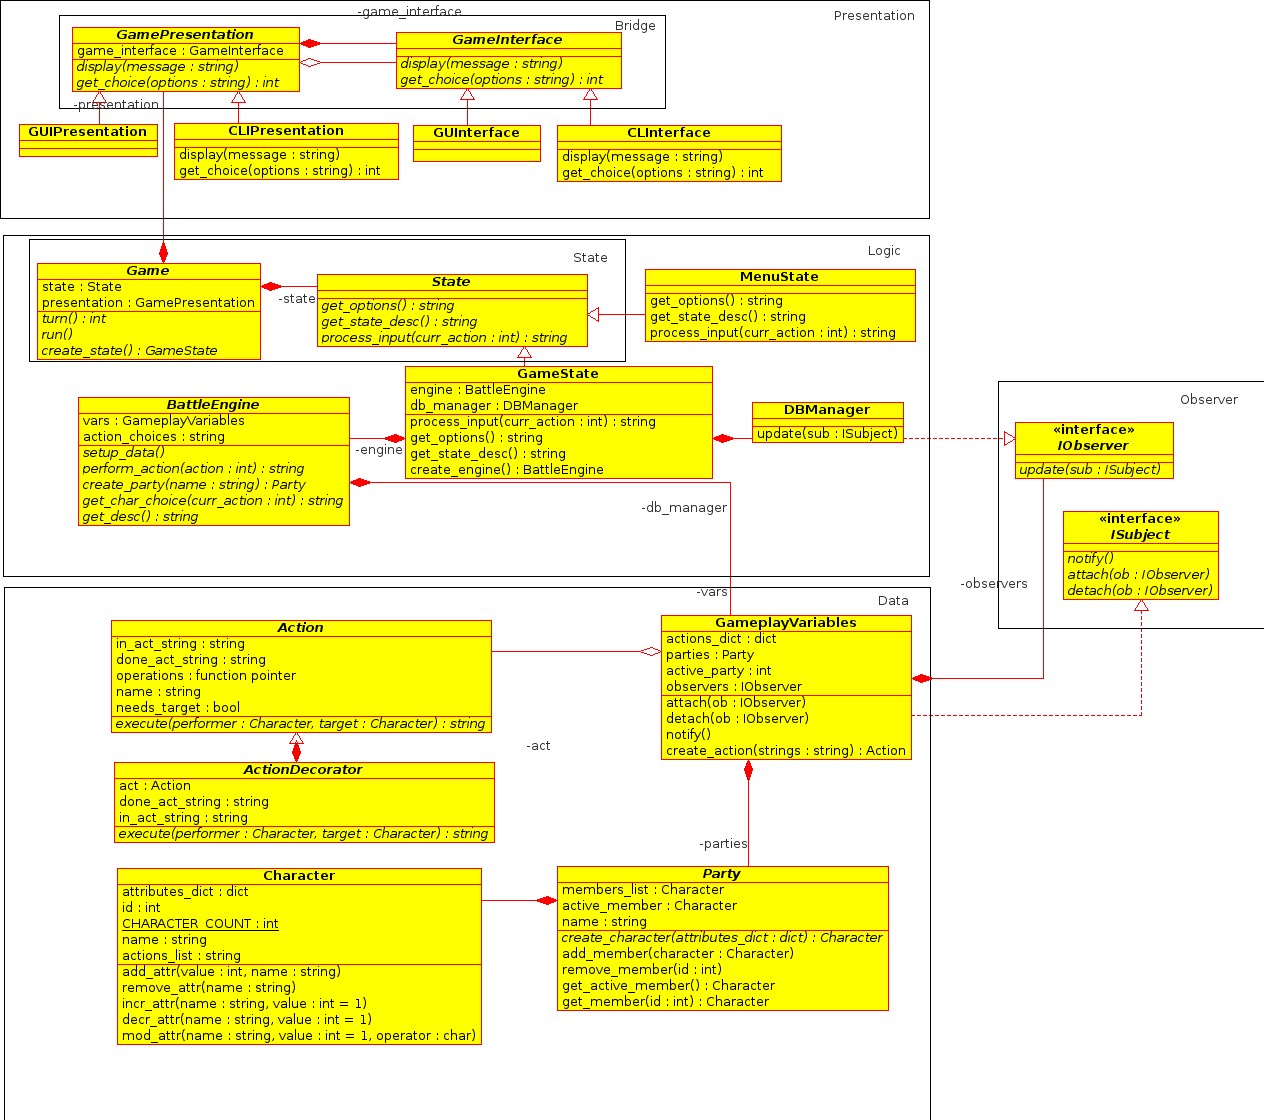
\includegraphics[scale=0.5]{pyturn.png}
\caption{pyturn package}
\label{pyturn package}
\end{figure}
\pagebreak
\section{Code}
\begin{verbatim}
from pyturn.data.Character import Character

class Action(object):

    """
     Represents an action performed by a Character on a Character

     @author: Max Vizard
    """

    """ ATTRIBUTES

     The string to display during the action

    in_act_str  (private)

     The string to display after the action

    done_act_str  (private)

     List of function pointers to functions that make up the action

    operations  (private)

     Name of action

    name  (private)

    """

    def execute(self, performer, target):
        """
         Perform the action. Semantically, performer performs the action on target.

         @type performer: Character
         @param performer: The Character who will be the semantic performer of the action
         @type target: Character
         @param target: The Character upon whom the action should be performed, if any
         @rtype: list
         @return: A list of strings representing the information about the action
         @author: Max Vizard
        """
        pass

    def get_operations(self):
        """
         Accessor method for operations attribute.
         @rtype: list
         @return: The list of operations
         @author: Max Vizard
        """
        pass

    def get_in_act(self):
        """
         Accessor method for in_act_str attribute.
         
         @rtype: string
         @return: The in_act_str attribute
         @author: Max Vizard
        """
        pass

    def get_done_act(self):
        """
         Accessor method for done_act_str attribute.
         
         @rtype: string
         @return: The done_act_str attribute
         @author: Max Vizard
        """
        pass
    
    def get_needs_target(self):
        """
         Accessor method for needs_target attribute.
         
         @rtype: boolean
         @return: Whether the Action needs a target
         @author: Max Vizard
        """
        pass
from pyturn.data.Action import Action
from pyturn.data.Character import Character


class ActionDecorator (Action):

    """
     Decorates an Action with additional functionality

    @author: Max Vizard
    """

    """ ATTRIBUTES

     The Action being decorated

    act  (private)

     The string to display after the action

    done_act_string  (private)

     The string to display during the action

    in_act_string  (private)

    """

    #def __init__(self, action):
    #    self.act = action

    def execute(self, performer, target=None):
        """
         Perform the action. Semantically, performer performs the action on
         target.

         @type performer: Character
         @param performer: The Character who will be the semantic
                                performer of the action
         @type target: Character
         @param target: The Character upon whom the action should be
                                performed, if any
         @rtype: list
         @return: A list of strings representing the information about
                        the action
         @author: Max Vizard
        """
        pass
        #return self.act.execute(performer, target)

    def get_operations(self):
        """
         Accessor method for operations attribute.
         
         @rtype: list
         @return: The list of operations
         @author: Max Vizard
        """
        pass

    def get_in_act(self):
        """
         Accessor method for in_act_str attribute.
         
         @rtype: string
         @return: The in_act_str attribute
         @author: Max Vizard
        """
        pass

    def get_done_act(self):
        """
         Accessor method for done_act_str attribute.
         
         @rtype: string
         @return: The done_act_str attribute
         @author: Max Vizard
        """
        pass

    def get_needs_target(self):
        """
         Accessor method for needs_target attribute.
         
         @rtype: boolean
         @return: Whether the Action needs a target
         @author: Max Vizard
        """
        passimport operator as operate

class Character:

    """
     Stores and manages data relating to an individual character and their attributes

     @author: Max Vizard
    """

    """ ATTRIBUTES

     A dict of all the character's attributes

    attributes_dict  (protected)
    
    A list of strings representing Actions this Character can perform
    
    actions_list (private)

     Unique identifier of the character

    id  (public)

     Static counter to keep track of how many characters have been created - used to
     assign IDs

    CHARACTER_COUNT  (private)

     The Character's name

    name  (private)

    """
    
    CHARACTER_COUNT = 0
    
    def __init__(self, name, attr_dict={'HP': 10, 'DF': 3, 'AD': 1}, actions=[]):
        self.name = name
        self.attributes_dict = attr_dict
        self.id = Character.CHARACTER_COUNT
        self.actions_list = actions
        Character.CHARACTER_COUNT += 1

    def get_action(self, a_int):
        """
         Gets the action represented by the input
         
         @type a_int: int
         @param a_int: An integer representing an Action
         @rtype: Action
         @return: The Action represented by the input
         @author: Max Vizard
        """
        return self.actions_list[a_int]
    
    def get_state(self):
        """
         Gets the current state of the Character
         
         @rtype: list
         @return: A list of strings representing the Character's
                     current state
         @author: Max Vizard
        """
        a = []
        for i in self.attributes_dict:
            a.append(i+" "+str(self.attributes_dict[i]))
        return a

    def remove_attr(self, name):
        """
         Remove an attribute from the character's dict

         @type name: string
         @param name: Name of attribute to remove
         @author: Max Vizard 
        """
        del self.attributes_dict[name]

    def incr_attr(self, name, value = 1):
        """
         Increase value of an attribute in the character's dict

         @type name: string
         @param name: Name of attribute
         @type value: int
         @param value: Value to increase the attribute by
         @author: Max Vizard
        """
        try:
            self.attributes_dict[name] += value
        except ValueError:
            print 'Expected a numerical value'

    def decr_attr(self, name, value = 1):
        """
         Decrease value of an attribute in the character's dict

         @type name: string
         @param name: Name of attribute to decrease
         @type value: int
         @param value: Value to decrease attribute by
         @author: Max Vizard
        """
        try:
            self.attributes_dict[name] -= value
        except ValueError:
            print 'Expected a numerical value'
            

    def mod_attr(self, name, value = 1, operator='+'):
        """
         Change value of an attribute in the character's dict using an operator

         @type name: string
         @param name: Name of attribute to modify
         @type value: int
         @param value: Value to modify the attribute by
         @type operator: char
         @param operator: Operator to modify the attribute by
         @author: Max Vizard
        """
        op_dict = {'+': operate.add,'-': operate.sub, '*': operate.mul, '/': operate.div }
        try:
            self.attributes_dict[name] = op_dict[operator](self.attributes_dict, value)
        except ValueError:
            print 'Expected a numerical value' 

    def add_attr(self, value, name):
        """
         Add an attribute to the character's dict

         @type value: int
         @param value: Value of attribute
         @type name: string
         @param name: Name of attribute
         @author: Max Vizard
        """
        if not self.attributes_dict[name]:
            self.attributes_dict[name] = value
        else:
            print 'Attribute already exists'
        
    def dead(self):
        if self.attributes_dict.get('popularity') < 25:
            return Truefrom pyturn.observer.ISubject import ISubject


class GameplayVariables (ISubject):

    """
     Holds all the Party instances in the current game, and various gameplay
     constants

    :author: Max Vizard
    """

    """ ATTRIBUTES

     Dict of all possible Actions

    actions_dict  (public)

     List of Party instances in the current game

    parties  (public)

     Integer representing the currently active Party

    active_party  (public)

     List of IObserver instances to notify when something changes

    observers  (public)

    """
    
    def __init__(self):
        self.actions_dict = {}
        self.parties = []
        self.active_party = -1
        self.observers = []
        
    def get_action(self, a_int):
        """
         Return an Action instance represented by the input, relative to
         the active Character of the active Party.
         
         @type a_int: int
         @param a_int: The index of the Action in the Character's own list
         @rtype: Action
         @return The Action at that position in the Character's list
        """
        party = self.parties[self.active_party]
        char = party.get_active_member()
        a_string = char.get_action(a_int)
        #print a_string
        return self.actions_dict.get(a_string)

    def attach(self, ob):
        """
         Add an IObserver to the observer list

        @param IObserver ob : IObserver to add to the observer list
        @return void :
        @author
        """
        self.observers.append(ob)

    def detach(self, ob):
        """
         Remove an IObserver from the observer list

        @param IObserver ob : IObserver to remove from the observer list
        @return void :
        @author
        """
        self.observers.remove(ob)

    def notify(self):
        """
         Call update() on all observers

        @return void :
        @author
        """
        for observer in self.observers:
            observer.update(self)




from pyturn.data.Action import Action
from pyturn.data.Character import Character


class ModAttribute (Action):

    """
     Increase an attribute of a Character

    :author: Max Vizard
    """

    """ ATTRIBUTES

     String to display during the action
     
    in_act_str  (private)

     The string to display after the action is finished

    done_act_str  (private)

     List of operations that make up the Action

    operations  (private)

    Name of the attribute in the Character attributes

    attr_str  (private)

     How much to change the attribute by

    value  (private)

     Name of action

    name  (private)
    
     Bool to indicate whether action expects target or not

    needs_target  (public)

    """

    def __init__(self,
                 name,
                 str_dict={'in': '', 'done': ''},
                 attr_str='',
                 value=0,
                 needs_target=False):

        self.name = name
        self.in_act_str = str_dict.get('in', '')
        self.done_act_str = str_dict.get('done', '')
        self.operations = [Character.incr_attr]
        self.attr_str = attr_str
        self.value = value
        self.needs_target = needs_target

    def execute(self, performer, target=None):
        """
         Do the action: Semantically, the performer is performing the action on
         the target

        @param Character performer : The Character performing the action
        @param Character target : The target of the action
        @return list : List of strings containing output about the action
        @author
        """
        results = ["display"]
        
        format_dict = {'performer': performer.name,
                       'attr': self.attr_str,
                       'value': abs(self.value)}

        if target:
            format_dict['target'] = target.name
            self.operations[0](target, self.attr_str, self.value)
            results.append(self.in_act_str.format(**format_dict))
            results.append(self.done_act_str.format(**format_dict))
        else:
            self.operations[0](performer, self.attr_str, self.value)
            results.append(self.in_act_str.format(**format_dict))
            results.append(self.done_act_str.format(**format_dict))

        return results

    def get_operations(self):
        """
         Accessor method for operations attribute.
         
        @return list : The list of operations
        @author
        """
        return self.operations[:] # Returns a copy instead of actual attribute

    def get_in_act(self):
        """
         Accessor method for in_act_str attribute.
         
        @return string : The in_act_str attribute
        @author
        """
        return self.in_act_str[:] # Returns a copy instead of actual attribute

    def get_done_act(self):
        """
         Accessor method for done_act_str attribute.
         
        @return string : The done_act_str attribute
        @author
        """
        return self.done_act_str[:] # Returns a copy instead of actual attribute
    
    def get_needs_target(self):
        """
         Accessor method for needs_target attribute.
         
        @return boolean : Whether the Action needs a target
        @author
        """
        return self.needs_target
from pyturn.observer.ISubject import ISubject
import Character

class Party (ISubject, ISubject):

    """
     Stores a list of members and manages member creation and retrieval

    :author: Max Vizard
    """

    """ ATTRIBUTES

     List of members

    members_list  (protected)

     The currently active member

    active_member  (protected)

    """

    def create_character(self, name, attributes_dict):
        """
         Factory method to create Character instances
         
        @param string name : String representing the name of the Character to be created
        @param dict attributes_dict : Dict of attributes for the new Character
        @return Character :
        @author
        """
        pass

    def add_member(self, character):
        """
         Add a Character to the list of members

        @param Character character : Character instance to add to the member list
        @return  :
        @author
        """
        pass

    def remove_member(self, id_num):
        """
         Remove a Character from the member list

        @param int id_num : ID of member to remove
        @return  :
        @author
        """
        pass

    def get_active_member(self):
        """
         Get the active member of this Party

        @return Character :
        @author
        """
        pass

    def get_member(self, id_num):
        """
         Get the Character instance that has the given ID if it is a member of this Party

        @param int id : The ID of the Character to get
        @return Character :
        @author
        """
        pass
    
    def get_state(self):
        """
         Get information about the state of this Party
         
         @return list : A list of strings representing the state of the Party
         @author
        """
        pass 

from Party import Party
from Character import Character

class PoliticalParty (Party):

    """
     A Party of politicians

    :author: Max Vizard
    """
    """ ATTRIBUTES
    
     Name of the party
    name  (public)

     List of members

    members_list  (private)

     The currently active member

    active_member  (private)

    """
    
    def __init__(self, name):
        self.name = name
        self.members_list = []
        self.active_member = None
        
    def create_character(self, name, attributes_dict, actions_list):
        """
         Factory Method to create a new Character
        
        @param string name : String representing the name of the Character to be created
        @param dict attributes_dict : Dictionary holding all the attributes of the new Character
        @return Character :
        @author
        """
        return Character(name, attributes_dict, actions_list)

    def add_member(self, politician):
        """
         Add a politician to the PoliticalParty

        @param Character politician : The Character to add to the PoliticalParty
        @return void :
        @author
        """
        self.members_list.append(politician)

    def remove_member(self, id_num):
        """
         Remove a member from the PoliticalParty

        @param int id_num : Integer representing the Character to remove
        @return void :
        @author
        """
        member = self.get_member(id_num)
        if member:
            self.members_list.remove(member)
        else:
            print 'Member with ID: %i not in party %s' % (id, self.name)

    def get_active_member(self):
        """
         Get the active member of the PoliticalParty

        @return Character : The active member of the party to be returned
        @author
        """
        return self.active_member

    def set_active_member(self, active):
        """
         Set the active member of the PoliticalParty
         
        @param Character active : The Character to set as active
        @return void :
        @author: 
        """
        self.active_member = active

    def get_member(self, id_num):
        """
         Return a Character with the ID specified

        @param int id_num : Integer representing the Character
        @return Character : The Character with the ID value specified or None if not found
        @author
        """
        for mem in self.members_list:
            if mem.id == id_num:
                return mem
            
        print 'Member with ID: %i not found' % id_num
        return None
        
    def dead(self):
        for mem in self.members_list:
            if not mem.dead():
                return False
        return True
        
    def get_state(self):
        """
         Get information about the state of this Party
         
         @return list : A list of strings representing the state of the Party
         @author
        """
        a = []
        for mem in self.members_list:
            if(mem.dead()):
                a.append(mem.name + " is out of the running!")
            else:
                a.append(mem.name + "\n")
                a.extend(mem.get_state())
        return a
from pyturn.data.ActionDecorator import ActionDecorator
from pyturn.data.Character import Character

class WithBackfire(ActionDecorator):
    """
     Changes an Action to also have a negative effect on the performer,
     for half the value of the action itself on the same attribute.

    :author: Max Vizard
    """

    """ ATTRIBUTES

     The Action being decorated

    act  (private)

     The string to display after the action

    done_act_string  (private)

     The string to display during the action

    in_act_string  (private)

     Name of action

    name  (private)

    """

    def __init__(self, action):
        #ActionDecorator.__init__(action)
        self.act = action

    def execute(self, performer, target=None):
        """
         Perform the action. Semantically, performer performs the action on
         target.

        @param Character performer : The Character who will be the semantic
                                     performer of the action
        @param Character target : The Character upon whom the action should be
                                  performed, if any
        @return string : A list of strings representing the information about
                         the action
        @author
        """
        pre_results = self.act.execute(performer, target)
        format_dict = {'performer': performer.name,
                       'attr': self.act.attr_str,
                       'value': abs(self.act.value) / 2}
        
        if target:
            format_dict['target'] = target.name
        
        try:
            pre_results[1] += ' However, this backfires and negatively affects {performer}.'
            pre_results[2] += ' {performer}\'s {attr} also reduced by {value} points!'
            
            pre_results[1] = pre_results[1].format(**format_dict)
            pre_results[2] = pre_results[2].format(**format_dict)
            performer.decr_attr(self.act.attr_str, abs(self.act.value) / 2)

            return pre_results

        except IndexError:
            print 'Expected at least two result strings from Action'
            print self.act.name

    def get_operations(self):
        """
         Accessor method for operations attribute.
         
        @return list : The list of operations
        @author
        """
        op = self.act.get_operations()
        op.extend(Character.decr_attr)
        return op

    def get_in_act(self):
        """
         Accessor method for in_act_str attribute.
         
        @return string : The in_act_str attribute
        @author
        """
        in_act = self.act.get_in_act()
        in_act += ' This backfires and negatively affects {performer}.'
        return in_act
        

    def get_done_act(self):
        """
         Accessor method for done_act_str attribute.
         
        @return string : The done_act_str attribute
        @author
        """
        done_act = self.act.get_done_act()
        done_act += ' {performer}\'s {attr} fell {value} points.'
        return done_act

    def get_needs_target(self):
        """
         Accessor method for needs_target attribute.
         
        @return boolean : Whether the Action needs a target
        @author
        """
        return self.act.get_needs_target()from pyturn.data.Party import Party
from pyturn.data.GameplayVariables import GameplayVariables

class BattleEngine(object):

    """
     Class that stores and manages interactions between parties, characters and
     actions. Bridges Data and Logic layers.

    :author: James Heslin
    """

    """ ATTRIBUTES

     Holds all gameplay data

    vars  (private)

    """

    def setup_data(self):
        """
         Initialises all the Party, Character and Action instances

        @return  :
        @author
        """
        pass

    def perform_action(self, action):
        """
         Performs the action specified by the input

        @param string action : The action to be performed
        @return string :
        @author
        """
        pass

    def create_party(self, name):
        """
         Interface for the creation of new Party instances

        @param string name : Name of the party
        @return Party :
        @author
        """
        pass

    def get_char_choice(self, curr_action):
        """
         Returns a list of all the characters the current action can be performed on.

        @param int curr_action : Integer representing the current action
        @return string :
        @author
        """
        pass



from pyturn.observer.IObserver import IObserver
import copy

class DBManager (IObserver):

    """
     Manages the saved state (in database or otherwise) of the game

    :author: James Heslin
    """

    def __init__(self, init_sub):
        self.last_sub = copy.deepcopy(init_sub)

    def update(self, sub):
        """
         Called by the IObserver's notify() method

        @param ISubject sub : Subject to check
        @return  :
        @author
        """
        self.last_sub = copy.deepcopy(sub)
        
        # print 'Update called on DB_Manager'
    
    def __str__(self):
        return str(self.__dict__)

    def __cmp__(self, other): 
        return self.__dict__ == other.__dict__


from BattleEngine import BattleEngine
from pyturn.data.PoliticalParty import PoliticalParty
from pyturn.data.GameplayVariables import GameplayVariables
from pyturn.data.ModAttribute import ModAttribute
from pyturn.data.WithBackfire import WithBackfire
from pyturn.logic.DBManager import DBManager
from pyturn.logic.Game import *

class ElectionEngine (BattleEngine):

    """
     Runs the election

    :author: James Heslin
    """
    """ ATTRIBUTES

     Holds all gameplay data

    vars  (private)

    """
    
    def __init__(self):
        self.vars = None
        self.setup_data()

    def setup_data(self):
        """
         Sets up data for ElectionGame

        @return  :
        @author
        """
        # setup subject and observer
        self.vars = GameplayVariables()
        self.db = DBManager(self.vars)
        self.vars.attach(self.db)
        
        
        partyA = self.create_party("Republicans")
        charA = partyA.create_character("Mitt Romney", {'popularity':50, 'entourage':500,
                                                        'investment':1000},
                                        ["Appeal", "Defame", "Lie"])
        partyA.add_member(charA)
        partyA.set_active_member(charA)
        
        partyB = self.create_party("Democrats")
        charB = partyB.create_character("Barack Obama", {'popularity':50, 'entourage':500,
                                                         'investment':1000},
                                        ["Legislate", 
                                         "Publish Birth Certificate", 
                                         "Respond To Disaster"])
        partyB.add_member(charB)
        partyB.set_active_member(charB)
        
        self.vars.parties.append(partyA)
        self.vars.parties.append(partyB)

        self.vars.active_party = 1
        
        action1 = ModAttribute("Appeal", {'in':"{performer} is appealing to the rich!", 
            'done':"{performer} appealed to the rich! His {attr} has increased by {value}!"}, 
                                    'popularity', 10, False)
        action2 = ModAttribute("Defame", {'in':"{performer} is insulting {target} publicly!", 
            'done':"{target}'s {attr} has fallen by {value}!"}, 
                                    'popularity', -10, True)
        action3 = ModAttribute("Lie", {'in':"{performer} is lying to the public about {target}'s policy!", 
            'done':"{performer} lied to the public about {target}! {target}\'s {attr} has decreased by {value}!"}, 
                                    'entourage', -50, True)
        action4 = ModAttribute("Legislate", {'in':"{performer} is legislating to make {target} and his rich friends pay for everyone's healthcare!", 
            'done':"{performer} appealed to the middle classes! His {attr} has increased by {value}!"}, 
                                    'popularity', 10, True)
        action5 = ModAttribute("Publish Birth Certificate", {'in':"{performer} is showing {target} up by proving he's American!", 
            'done':"{target}'s {attr} has fallen by {value}!"}, 
                                    'popularity', -10, True)
        action6 = ModAttribute("Respond To Disaster", {'in':"{performer} is responding to Hurricane Sandy by volunteering to help with relocation!", 
            'done':"{performer} impressed the public, but his {attr} have less to do so they have decreased by {value}!"}, 
                                    'entourage', -50, False)
        
        # decorate the Lie action
        action3 = WithBackfire(action3)
        
        
        actions = {'Appeal':action1, 'Defame':action2, 'Lie':action3,
                   'Legislate':action4, 'Publish Birth Certificate':action5,
                   'Respond To Disaster':action6}
        self.vars.actions_dict = actions
        
        self.vars.notify()
        
        # GAAAME ON!

    def perform_action(self, action):
        """
         Performs an action

        @param int action : An integer representing the action to be performed
        @return list : List of strings representing the results, with a flag
                       in index 0 representing the type of result
        @author
        """
        self.vars.notify()
        
        act = self.vars.get_action(action)
        active_party = self.vars.parties[self.vars.active_party]
        performer = active_party.get_active_member()
        target = None
        # Hypothetically, we would call get_char_choice here somehow
        
        if act.get_needs_target():
            #print "Needs target"
            if len(self.vars.parties) == 2:
                for i in xrange(len(self.vars.parties)):
                    if not i == self.vars.active_party:
                        target_party = self.vars.parties[i]
                        target = target_party.get_active_member()
                       
            else:
                # Code for three or more parties here
                pass
            
        return (self.execute(act, performer, target))

    def execute(self, act, performer, target=None):
        """
         Do the action: Semantically, the performer is performing the action on the
         target

        @param Character performer : The Character performing the action
        @param Character target : The target of the action
        @return list : List of strings containing output about the action
        @author
        """
        return act.execute(performer, target)


    def create_party(self, name):
        """
         Factory method to create a new Party

        @param string name : The name of the party
        @return Party :
        @author
        """
        return PoliticalParty(name)
    
    def get_options(self):
        char = self.vars.parties[self.vars.active_party].get_active_member()
        ch_act =[CHOOSE_FLAG]
        ch_act.extend(char.actions_list)
        #print ch_act
        return ch_act

    def dead(self):
        """
         Method to check if all members of the Party are 'dead'
        
        @return bool : Whether all members are dead
        @author
        """
        for i in self.vars.parties:
            if i.dead():
                return [i.name + " are now out of the race!"]

    def end_turn(self):
        """
         Method to be called at the end of each turn
         
        @return list : A list containing a number and possibly a message
        """
        d = self.dead()
        if d is not None:
            # GAME OVER MAN, GAME OVER
            self.vars.detach(self.db)
            res = [-1]
            res.extend(d)
            #print res
            return res
        if self.vars.active_party < len(self.vars.parties) -1:
            self.vars.active_party = self.vars.active_party+1
        else:
            self.vars.active_party = 0
        return [1]
            
    def get_desc(self):
        """
         Method to get the state of the active party
        
        @return list : Information about the state of the active party
        """
        return self.vars.parties[self.vars.active_party].get_state()

# NOT USING THIS YET - It's wrong
    def get_char_choice(self, curr_action):
        """
         Get a list of the choices available as targets of the current action

        @param string curr_action : A string representing the current action
        @return string :
        @author
        """
        char = self.vars.parties[self.vars.active_party].get_active_member()
        return char.actions_list[curr_action]


from Game import Game, SWITCH_FLAG, CHOOSE_FLAG, DISPLAY_FLAG, QUIT_FLAG
from GameState import GameState
from MenuState import MenuState
from pyturn.presentation.CLIPresentation import CLIPresentation
#from pyturn.presentation.GUIPresentation import GUIPresentation
from sys import exit


class ElectionGame (Game):

    """
     Main Class for the Election game

    :author: James Heslin
    """

    """ ATTRIBUTES

     Holds the current state of the application

    states  (private)

     Holds a reference to the current GamePresentation instance

    presentation  (private)

    """

    def __init__(self):
        self.states = [self.create_state('menu'), self.create_state('game')]
        self.presentation = CLIPresentation()
        #self.presentation = GUIPresentation()
    def turn(self):
        """
         Method to call each turn in the Election game

        @return int: flag to tell the run method what to do next
        @author
        """
        opt = self.states[0].get_options()
        #print self.states[0]
        #print opt
        inp = self.presentation.get_choice(opt[1:])
        result = self.states[0].process_input(inp)
        while (result[0] == CHOOSE_FLAG):
            inp = self.presentation.get_choice(result[1:])
            result = self.states[0].process_input(inp)
        if(result[0] == QUIT_FLAG):
            self.presentation.display(result[1:])
            return -1
        elif(result[0] == SWITCH_FLAG):
            self.presentation.display(result[1:])
            return 1
        elif(result[0] == DISPLAY_FLAG):
            self.presentation.display(result[1:])
            return 0
        

    def run(self):
        """
         Main loop for the Election game

        @author
        """
        turn_flag = 0
        while not(turn_flag == -1):
            try:
                turn_flag = self.turn()
                if turn_flag == 1:
                    # Switch state
                    tmp = self.states[0]
                    self.states[0] = self.states[1]
                    self.states[1] = tmp
                elif turn_flag == -1:
                    # Quit
                    exit(0)              
                  
                end = self.states[0].end_turn()
                if end is not None and end[0] == -1:
                    end.extend(["Game over, man!", "GAME OVER!"])
                    self.presentation.display(end)
                    exit(0)
                self.presentation.display(self.states[0].get_state_desc())
            except ValueError:
                self.presentation.display(["Invalid input!"])
            except IndexError:
                self.presentation.display(["Invalid action!"])

    def create_state(self, s_type):
        """
         Create a state

        @return State : an instance of a subclass of State
        @author
        """
        
        if s_type == 'game':
            return GameState()
        elif s_type == 'menu':
            return MenuState()
        

if __name__ == "__main__":
    e_g = ElectionGame()
    e_g.run()

from State import State
from GameState import *
from pyturn.presentation.GamePresentation import GamePresentation

SWITCH_FLAG = "switch"
QUIT_FLAG = "quit"
CHOOSE_FLAG = "choose"
DISPLAY_FLAG = "display"

class Game:

    """
     Main class for the application

    :author: James Heslin
    """

    """ ATTRIBUTES

     Holds the current state of the application

    state  (private)

     Holds a reference to the current GamePresentation instance

    presentation  (private)

    """

    def turn(self):
        """
         Method that is called every iteration of the run loop, returns 0 to change
         state, -1 to quit

        @return int :
        @author
        """
        pass

    def run(self):
        """
         Main game loop, calls turn until turn returns quit value

        @return  :
        @author
        """
        pass

    def create_state(self):
        """
         Factory method providing an interface for creating State instances

        @return GameState :
        @author
        """
        pass



from State import State
from BattleEngine import BattleEngine
from ElectionEngine import ElectionEngine
from DBManager import DBManager


class GameState (State):

    """
     State representing the 'play'-specific processes

    :author: James Heslin
    """

    """ ATTRIBUTES

     Instance of BattleEngine specific to this GameState

    engine  (private)

     The data manager for this game state
     

    db_manager  (private)

    """
    
    def __init__(self):
        self.engine = self.create_engine()
        #self.db_manager = DBManager()

    def get_options(self):
        """
         Return the names of the currently available actions as a list of strings

        @return list : List of possible actions, first element is a flag 
        @author
        """
        return self.engine.get_options()

    def get_state_desc(self):
        """
         Returns a description of the current game state

        @return string :
        @author
        """
        return self.engine.get_desc()

    def create_engine(self):
        """
         Interface for the creation of new BattleEngine instances

        @return BattleEngine : A subclass of BattleEngine for this GameState
        @author
        """
        return ElectionEngine()

    def process_input(self, curr_action):
        """
         Performs the current action and returns the result

        @param int curr_action : An integer representing the current action
        @return string : 
        @author
        """
        return self.engine.perform_action(curr_action)

    def end_turn(self):
        """
         Finish the current turn.
        @author
        """
        return self.engine.end_turn()


from State import *
from pyturn.logic.Game import SWITCH_FLAG, CHOOSE_FLAG, DISPLAY_FLAG, QUIT_FLAG

class MenuState (State):

    """
     Menu-specific behaviour
    
    :author: James Heslin
    """

    def get_options(self):
        """
         Get the currently available menu options

        @return string :
        @author
        """
        return [CHOOSE_FLAG, "Start game", "Quit"]

    def get_state_desc(self):
        """
         Returns a string describing the current state of the menu

        @return string :
        @author
        """
        return [DISPLAY_FLAG, "Menu"]

    def process_input(self, curr_action):
        """
         Process the input to the menu

        @param int curr_action : 
        @return string :
        @author
        """
        if curr_action == 0:
            return [SWITCH_FLAG, "Starting game..."]
        elif curr_action == 1:
            return [QUIT_FLAG, "Quitting..."]
        else:
            return ["DERP", "DERP"]

    def end_turn(self):
        """
         Finish the current turn.
        @author
        """
        pass

class State(object):

    """
     Interface for state-specific behaviour

    :author: James Heslin
    """

    def _get_options(self):
        """
         Get the currently available state-specific options

        @return string :
        @author
        """
        pass
    
    def end_turn(self):
        """
         Finish the current turn.
        @author
        """
        pass

    def _get_state_desc(self):
        """
         Returns a string describing the state

        @return string :
        @author
        """
        pass

    def _process_input(self, curr_action):
        """
         Process input in a state-specific way

        @param int curr_action : 
        @return string :
        @author
        """
        pass



class IObserver:

    """
     Defines Observer interface

    :author: Max Vizard
    """

    def update(self, sub):
        """
         Action taken when a subject notifies observer of change

        @param ISubject sub : Instance of the subject that changed
        @return void :
        @author
        """
        pass



class ISubject:

    """
     Defines Subject interface

    :author: Max Vizard
    """

    def notify(self):
        """
         Calls update() on all the observers.

        @return void :
        @author
        """
        pass

    def attach(self, ob):
        """
         Add an observer to the list

        @param IObserver ob : The IObserver instance to add to the list
        @return void :
        @author
        """
        pass

    def detach(self, ob):
        """
         Remove an observer from the list

        @param IObserver ob : The IObserver instance to remove from the list
        @return void :
        @author
        """
        pass



from GamePresentation import GamePresentation
from CLInterface import CLInterface

class CLIPresentation (GamePresentation):

    """
     Implementation of GamePresentation that has CLInterface as its interface

    :author: James Heslin (PROGRAM_IX)
    """
    
    def __init__(self):
        self.game_interface = CLInterface()

    def display(self, message):
        """
         Implementation of display that delegates to its CLInterface instance

        @param string message : Message to be passed to CLInterface
        @return  :
        @author
        """
        self.game_interface.display(message)

    def get_choice(self, options):
        """
         Implementaion of get_choice that delegates to its CLInterface instance

        @param string options : List of options to pass to the CLInterface 
        @return int :
        @author
        """
        return self.game_interface.get_choice(options)



from GameInterface import GameInterface

class CLInterface (GameInterface):

    """
     Command Line Interface to game

    :author: James Heslin (PROGRAM_IX)
    """

    def display(self, message):
        """
         Prints the message to the command line

        @param string message : Message to be displayed
        @return  :
        @author
        """
        for i in message:
            print i

    def get_choice(self, options):
        """
         Lists the options in the CLI and returns  the user input

        @param string options : List of options to present to the user
        @return int :
        @author
        """
        n = 1
        for o in options:
            print n, "-", o
            n = n+1
        res = int(raw_input("Select an option: "))-1
        #print "Selected", res
        return res



from GamePresentation import *
from GUInterface import GUInterface

class GUIPresentation (GamePresentation):

    """
     Implementation of GamePresentation that has GUInterface as its interface

    :version:
    :author: James Heslin (PROGRAM_IX)
    """
    
    def __init__(self):
        self.game_interface = GUInterface()

    def display(self, message):
        """
         Implementation of display that delegates to its GUInterface instance

        @param string message : Message to be passed to GUInterface
        @return  :
        @author
        """
        self.game_interface.display(message)

    def get_choice(self, options):
        """
         Implementaion of get_choice that delegates to its GUInterface instance

        @param string options : List of options to pass to the GUInterface 
        @return int :
        @author
        """
        return self.game_interface.get_choice(options)



from GameInterface import GameInterface
import easygui as eg

class GUInterface (GameInterface):

    """
     Graphical interface to game

    :author: James Heslin
    """

    def display(self, message):
        """
         Prints the message to the command line

        @param string message : Message to be displayed
        @return  :
        @author
        """
        all_msg = ""
        for i in message:
            all_msg = all_msg + (i + "\n")
        eg.msgbox(all_msg, message[0])

    def get_choice(self, options):
        """
         Lists the options in the CLI and returns  the user input

        @param string options : List of options to present to the user
        @return int :
        @author
        """
        return options.index(eg.choicebox("Select an action", "Choice", 
                                          options))


from GamePresentation import *

class GameInterface(object):

    """
     Specifies the interface for user interaction with the game

    :author: James Heslin (PROGRAM_IX)
    """

    def display(self, message):
        """
         Displays the message to the user

        @param string message : Message to display
        @return  :
        @author
        """
        pass

    def get_choice(self, options):
        """
         Presents a list of choices to the user and returns their choice

        @param string options : List of options to present to the user
        @return int :
        @author
        """
        pass



from GameInterface import *

class GamePresentation:

    """
     Defines interface for presenting the game to the user

    :author: James Heslin (PROGRAM_IX)
    """

    """ ATTRIBUTES

     The instance of GameInterface to delegate to

    game_interface  (private)

    """


    def display(self, message):
        """
         Sends a message to the interface to be displayed

        @param string message : The message string to pass to the interface to be displayed
        @return  :
        @author
        """
        pass

    def get_choice(self, options):
        """
         Send a list of options to the game interface to display them to the user. The
         interface gets the user choice and this method returns it

        @param string options : List of options to pass to the interface to be presented to the user
        @return int :
        @author
        """
        pass




import unittest
from pyturn.data import Character


class TestCharacter(unittest.TestCase):

    def setUp(self):
        self.chell = Character('Chell', {'HP': 10, 'AD': 5, 'DF': 3})

    def test_inc_attr(self):
        base_health = self.chell.get_attr('HP')
        self.chell.inc_attr('HP', 5)

        self.assertEqual(self.chell.get_attr('HP'), base_health + 5)
import unittest
from pyturn.data.Character import Character
from pyturn.data.ModAttribute import ModAttribute
from pyturn.data.WithBackfire import WithBackfire


class decorator_test(unittest.TestCase):

    def setUp(self):
        self.tom = Character('Tom', {'HP': 10, 'AD': 5, 'DF': 3})
        self.dick = Character('Dick', {'HP': 10, 'AD': 5, 'DF': 3})
        self.decr_act = ModAttribute("Punch",
                                        {'in': "{performer} punched {target}!",
                                         'done': "{target}'s {attr} reduced by {value}!"},
                                        'HP', -4)

    def testUndecoratedAttack(self):
        #print 'ModAttribute.execute(Tom, Dick) \n'
        
        results = self.decr_act.execute(self.tom, self.dick)

        self.assertEqual(results[1], 'Tom punched Dick!')
        self.assertEqual(results[2], 'Dick\'s HP reduced by 4!')

    def testDecoratedAttack(self):
        self.assertEqual(self.dick.attributes_dict['HP'], 10)
        self.assertEqual(self.tom.attributes_dict['HP'], 10)
        
        print 'ModAttribute.execute(Tom, Dick) \n'
        act_with_backfire = WithBackfire(self.decr_act)
        results = self.decr_act.execute(self.tom, self.dick)
        
        print 'Results: \n'
        for res in results[1:]:
            print '\t' + res + '\n'
        
        self.assertEqual(self.dick.attributes_dict['HP'], 6)
        self.assertEqual(self.tom.attributes_dict['HP'], 10)

        print 'Decorating.. WithBackfire(ModAttribute)\n'
        results = act_with_backfire.execute(self.tom, self.dick)
        print 'Results: \n'
        for res in results[1:]:
            print '\t' + res + '\n'
            
        self.assertEqual(self.dick.attributes_dict['HP'], 2)
        self.assertEqual(self.tom.attributes_dict['HP'], 8)

if __name__ == "__main__":
    #import sys;sys.argv = ['', 'Test.testName']
    unittest.main()
import unittest
from pyturn.data.GameplayVariables import GameplayVariables
from pyturn.logic.DBManager import DBManager

from pyturn.data.Character import Character
from pyturn.data.PoliticalParty import PoliticalParty
from pyturn.data.ModAttribute import ModAttribute
from pyturn.data.WithBackfire import WithBackfire


class decorator_test(unittest.TestCase):

    def setUp(self):
        tom = Character('Tom', {'HP': 10, 'AD': 5, 'DF': 3})
        dick = Character('Dick', {'HP': 10, 'AD': 5, 'DF': 3})
        decr_act = ModAttribute("Punch",
                                        {'in': "{performer} punched {target}!",
                                         'done': "{target}'s {attr} reduced by {value}!"},
                                        'HP', -4)
        partA = PoliticalParty('Pirate Party')
        partA.add_member(tom)
        partA.add_member(dick)
        partA.set_active_member(tom)
                
        self.vars = GameplayVariables()
        self.vars.parties = [partA]
        self.vars.active_party = 0
        self.vars.actions_dict = {'Punch': decr_act}
        
    def testDecoration(self):
        self.db = DBManager(self.vars)
        
        print 'Attaching DBmanager to vars'
        self.vars.attach(self.db)
        
        dbs_last_subject = (self.db.last_sub, )
        #print vars(dbs_last_subject)
        self.vars.active_party = 666
        
        print 'Calling notify on self.vars'
        self.vars.notify()
        
        self.assertNotEqual(dbs_last_subject[0],
                         self.db.last_sub)
        print 'Asserted that DBManagers instance of vars has changed'
        

if __name__ == "__main__":
    #import sys;sys.argv = ['', 'Test.testName']
    unittest.main()
import unittest
from pyturn.presentation.CLIPresentation import CLIPresentation
from pyturn.presentation.GUIPresentation import GUIPresentation
from pyturn.presentation.CLInterface import CLInterface
from pyturn.presentation.GUInterface import GUInterface

class TestPresentation(unittest.TestCase):
    
    def setUp(self):
        self.pres_cli = CLIPresentation(CLInterface())
        self.pres_gui = GUIPresentation(GUInterface())

    def test_display(self):
        self.pres_cli.display("Some test message")
        self.pres_gui.display("Some test message")
        
    def test_choice(self):
        self.pres_cli.get_choice(["Test Action 1", "Test Action 2", 
                              "Test Action 3"])
        print self.pres_gui.get_choice(["Test Action 1", "Test Action 2", 
                              "Test Action 3"])

\end{verbatim}

\end{document}
